\section{Benchmark details}
Next, we have a closer look at some of the benchmarks and see how the effectiveness of each optimisation depends on the characteristics of the source code. The first section of Table \ref{tbl-performance-per-benchmark} shows the distribution of the JVM instructions executed in each benchmark, and both the maximum and average number of bytes on the JVM stack. We can see some important differences between the benchmarks. While the benchmarks on the left are almost completely load/store bounded, towards the right the benchmarks become more computation intensive, spending fewer instructions on loads and stores, and more on math or bitwise operations. The left benchmarks have only a few bytes on the stack, but as the benchmarks contain more complex expressions, the number of values on the stack increases.

The second part of tables \ref{tbl-performance-per-benchmark} and \ref{tbl-codesize-per-benchmark} first shows the overhead before optimisation, split up in the four instruction categories. We then list the effect of each optimisation on the total overhead. Finally we show the overhead per category after applying all optimisations.

The improved peephole optimiser and stack caching both target the push/pop overhead. Stack caching can eliminate almost all, and replaces the need for a peephole optimiser, but it is interesting to compare the two. The improved peephole optimiser does well for the simple benchmarks like sort and search, leaving less overhead to remove for stack caching. Moving to the right, the more complicated expressions mean there is more distance between a push and a pop, leaving more cases that cannot be handled by the peephole optimiser, and replacing it with stack caching yields a big improvement.

The benchmarks on the left spend more time on load/store instructions. This results in higher load/store overhead, and the two optimisations that target this overhead, popped value caching and mark loops, have a big impact. For the computation intensive benchmarks on the right, the load/store overhead is much smaller, but the higher stack size means stack caching is very important for these benchmarks.

The first seven benchmarks are smaller benchmarks that can highlight certain specific aspects of our approach, the CoreMark benchmark represents larger sensor node applications, and is a mix of different types of processing. As a result, it is an average case in almost every row in Table \ref{tbl-performance-per-benchmark}. The reason it ends up being the slowest after all optimisations was discussed in \ref{sec-evaluation-coremark-unfair-optimisations}. With the 'unfair' optimisations described there, CoreMark's performance overhead would be 61\%, very close to the average of the other benchmarks.

\paragraph{Bit shifts} Interestingly, the reason fft is the slowest, is similar to the reason rc5 is fastest: they both spend a large amount of time doing bit shifts. Rc5 shifts by a variable, but large number of bits. Only 8.0\% of the executed JVM instructions are bit shifts, but they account for 71\% of the execution time in the optimised version. For these variable bit shifts, our translator and \mycode{avr-gcc} generate a similar loop, so the two share a large constant factor.

On the other hand fft is a hard case because it does many constant shifts by exactly 6 bits. For these, our VM simply emits 6 single shifts, which is slower than the special case \mycode{avr-gcc} emits for shifts by exactly 6 bits.  While we could do the same, we feel this special case is too specific to include in our VM.

\paragraph{Bubble sort} Next we look at bubble sort in some more detail. After optimisation, we see most of the stack related overhead has been eliminated and of the 94.6\% remaining performance overhead, most is due to other sources. For bubble sort there is a single, clearly identifiable source. When we examine the detailed trace output, this overhead is largely due to \mycode{ADD} instructions, but bubble sort hardly does any additions. This is a good example of how the simple JVM instruction set leads to less efficient code. To access an array we need to calculate the address of the indexed value, which takes one move and seven additions for an array of ints. This calculation is repeated for each access, while the C version has a much more efficient approach, using the auto-increment version of the AVR's LD and ST instructions to slide a pointer over the array. Of the remaining 94.6\% overhead, 73\% is caused by these address calculations.

% Overhead from address calculations in bubble sort:
% For all IASTORE/IALOAD instructions (2 each):
% MOVW 130560
% ADC  391680
% ADD  391680
% ADIW 261120
% total 1175040
% C 1589218
% overhead 1175040/1589218 = .739382514

\begin{figure}
 \centering
 \begin{minipage}{0.45\textwidth}
  \centering
  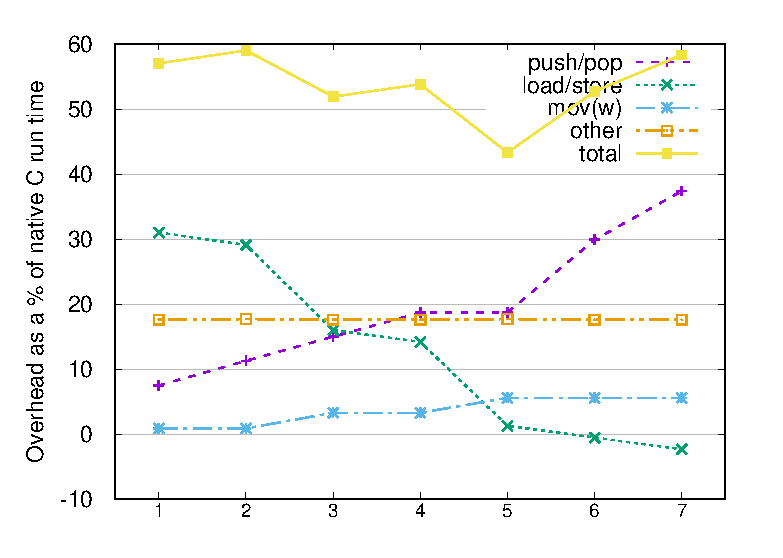
\includegraphics[width=\myfiguresizexxtea]{performance-pinnedregs-xxtea-per-opcode-category.eps}
  \caption{Xxtea performance overhead for different number of pinned register pairs}
  \label{fig-performance-pinnedregs-xxtea-per-opcode-category}
 \end{minipage}\hfill
 \begin{minipage}{0.45\textwidth}
  \centering
  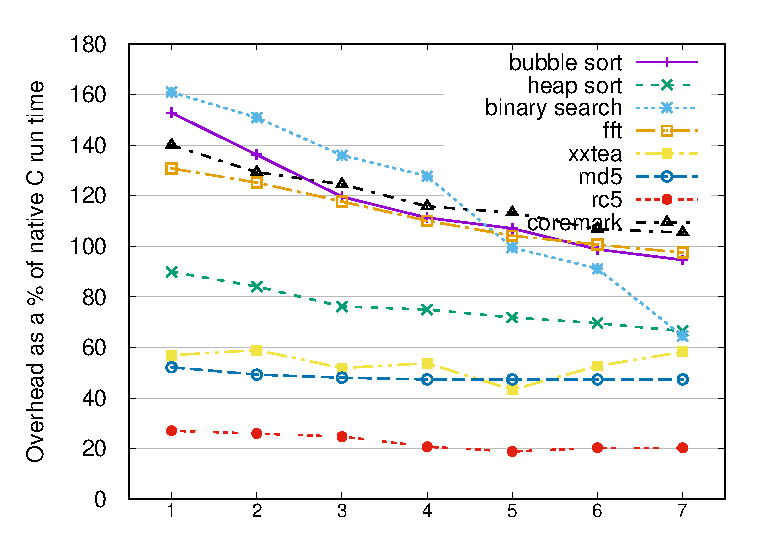
\includegraphics[width=\myfiguresizexxtea]{performance-pinnedregs-per-benchmark.eps}
  \caption{Per benchmark performance overhead different number of pinned register pairs}
  \label{fig-performance-pinnedregs-per-benchmark}
 \end{minipage}
\end{figure}

\paragraph{Xxtea and the mark loops optimisation} Perhaps the most interesting benchmark is xxtea. Its high average stack depth means popped value caching does not have much effect: most registers are used for real stack values, leaving few chances to reuse a value that was previously popped from the stack. 

When we apply the mark loops optimisation, performance actually degrades by 5.1\%, and code size overhead increases 6\%! Here we have an interesting tradeoff: if we use a register to pin a variable, accessing that variable will be cheaper, but this register will no longer be available for stack caching, so more stack values may have to be spilled to memory.

For most benchmarks the maximum of 7 register pairs to pin variables to was also the best option. At a lower average stack depth, the fewer number of registers available for stack caching is easily compensated for by the cheaper variable access. For xxtea however, the cost of spilling more stack values to memory outweighs the gains of pinning more variables when too many variables are pinned. Figure \ref{fig-performance-pinnedregs-xxtea-per-opcode-category} shows the overhead for xxtea from the different instruction categories. When we increase the number of register pairs used to pin variables from 1 to 7, the load/store overhead steadily decreases, but the push/pop and move overhead increase. The optimum is at 5 pinned register pairs, at which the total overhead is only 43\%, instead of 58\% at 7 pinned register pairs.

 Interestingly, when we pin 7 pairs, the AOT version actually does fewer loads and stores than the C compiler. Under high register pressure the C version may spill a register value to memory and later load it again, adding extra load/store instructions. When the AOT version pins too many registers, it will also need to spill values, but this adds push/pop instructions instead of loads/stores.

Figure \ref{fig-performance-pinnedregs-per-benchmark} shows the performance for each benchmark, as the number of pinned register pairs is increased. The three benchmarks that stay stable or even slow down when the number pinned pairs is increased beyond 5 are exactly the benchmarks that have a high stack depth: xxtea, md5 and rc5. It should be possible to develop a simple heuristic to allow the VM to make a better decision on the number of registers to pin. Since our current VM always pins 7 pairs, we used this as our end result and leave this heuristic to future work.

